\documentclass[11pt,a4paper]{article}

\usepackage{fancyheadings}
\usepackage{amsmath}
\usepackage{amssymb}
\usepackage{psfig}
\usepackage{here}
\usepackage{array}
\usepackage{graphicx}
\usepackage{eepic,epic}
\usepackage{alltt}
\usepackage[french]{babel}
% \usepackage[dvips]{epsfig}


\oddsidemargin -0.5cm
\evensidemargin -0.5cm
\topmargin -2.2cm
\textheight 22.7cm
\textwidth 17cm
\headheight 1.0cm

\newfont{\eufmtwelve}   {eufm10 scaled \magstep1}
\newfont{\eufmten}      {eufm10 }
\newfont{\eufmnine}     {eufm9 }
\newfont{\eufmeight}    {eufm8 }
\newfont{\eufmseven}    {eufm7 }
\newfont{\eufmsix}      {eufm6 }
\newfont{\eufmfive}     {eufm5 }
\newfont{\eusmtwelve}   {eusm10 scaled \magstep1}
\newfont{\eusmten}      {eusm10}
\newfont{\eusmnine}     {eusm9 }
\newfont{\eusmeight}    {eusm8 }
\newfont{\eusmseven}    {eusm7 }
\newfont{\eusmsix}      {eusm6 }
\newfont{\eusmfive}     {eusm5 }
\newfont{\msbmtwelve}   {msbm10 scaled \magstep1}
\newfont{\msbmeight}    {msbm8}

\newcommand{\udl}{\underline}
\newcommand{\udll}[1]{{\udl{\udl{#1}}}}
\newcommand{\udlll}[1]{{\udl{\udl{\udl{#1}}}}}
\newcommand{\Reel}{{\mbox{\msbmtwelve R}}}      % L'ensemble des reels.
\newcommand{\reel}{{\mbox{\msbmeight R}}}       % L'ensemble des reels.
\newcommand{\Rn}{\Reel^{n}}
\newcommand{\Rtrois}{\Reel^{3}}
\newcommand{\Complex}{\mbox{\msbmtwelve C}}     % L'ensemble des complexes.
\newcommand{\Naturel}{\mbox{\msbmtwelve N}}  % L'ensemble des entiers naturels.
\renewcommand{\emptyset}{\mbox{$\circ$\hspace{-.50em}/}}  % ensemble vide.
\newcommand{\Cont}{{\cal C}}            % L'ensemble des fonctions continues
\newcommand{\Cinf}{{\cal C}^{\infty}}   % L'ensemble des fonction C-infinies
\renewcommand{\vec}[1]{\overrightarrow{\!\!#1}}
\newcommand{\subsetcont}{{\subset\hspace{-.6em}_{\scriptscriptstyle >} }}
\newcommand{\Frac}[2]{{\ds \frac{\ds #1}{\ds #2}}}
\newcommand{\interior}[1]{{\stackrel{\circ}{#1}}}
\newcommand{\cqfd}{{\hfill\rule{2.5mm}{2.5mm}}}
\newcommand{\vectwo}[2]{{\left(\hspace{-.5em}\begin{array}{c} {#1} \\ {#2}
     \end{array}\hspace{-.5em}\right)}}
\newcommand{\vecthree}[3]{{\left(\hspace{-.5em}\begin{array}{c} {#1}
     \\ {#2} \\ {#3} \end{array}\hspace{-.5em}\right)}}
\newcommand{\vecfive}[5]{{\left(\hspace{-.5em}\begin{array}{c} {#1}
     \\ {#2} \\ {#3} \\ {#4} \\ {#5} \end{array}\hspace{-.5em}\right)}}
\def\infess{\mathop{\iflanguage{english}{\mbox{ess$\,$inf}}{\mbox{inf$\,$ess}}}}
\def\supess{\mathop{\iflanguage{english}{\mbox{ess$\,$sup}}{\mbox{sup$\,$ess}}}}
\def\essinf{\mathop{\iflanguage{english}{\mbox{ess$\,$inf}}{\mbox{inf$\,$ess}}}}
\def\esssup{\mathop{\iflanguage{english}{\mbox{ess$\,$sup}}{\mbox{sup$\,$ess}}}}
\def\aplim{\mathop{\mbox{ap$\,$lim}}}
\def\aplimsup{\mathop{\mbox{ap$\,$lim$\,$sup}}}
\def\apliminf{\mathop{\mbox{ap$\,$lim$\,$inf}}}
\def\convto{\mathop{\hbox{\rightarrowfill}}} % converge vers.
\newcommand{\rightgap}{{]\hspace{-0.12em}]}}
\newcommand{\leftgap}{{[\hspace{-0.12em}[}}
\newcommand{\gapof}[1]{{\leftgap {#1} \rightgap}}
\newcommand{\restrictiona}[1]
{{ \begin{picture}(13,10) \put(-1,-4){$\mid_{#1}$} \end{picture}
}} % Le signe "Restriction sur #1"

\def\Indic{\mbox{1\hspace{-0.20em}I}}   % Fonction l'indicatrice

\def\bar3{|\hspace{-1pt}\|} % 3bar verticaux pour les normes matricielles.
\def\fleche{\overrightarrow} %fleche en haut
\def\cvfaible{\rightharpoonup} %fleche cv faiblement
\def\longmapsto
{ \begin{picture}(0,10)
  \put(0,0){$\scriptstyle{\vdash}$} \end{picture} \mbox{$\longrightarrow$}
} 

\def\build#1_#2^#3{\mathrel{
 \mathop{\kern 0pt#1}\limits_{#2}^{#3}}} % Ecrire en dessous et dessus un symbole.

\def\Dist{\mbox{\eusmtwelve D}} %signe de distribution
\def\dist{\mbox{\eusmten D}} %signe de distribution


%definition de commandes utilses
\newcommand{\ds}{\displaystyle}
\newcommand{\rc}{{\par}}
\newcommand{\rcc}{{\par\medskip}}
\newcommand{\rccc}{{\par\bigskip}}


%definition des environnements theoreme, lemme, ...
\usepackage{boxedminipage}
% \newenvironment{largebox}
%   { \rc\noindent \begin{boxedminipage}[t]{\textwidth} }
%   { \end{boxedminipage}  \rccc\noindent }
\newenvironment{largebox}
  { \rc\noindent \begin{boxedminipage}[t]{\linewidth} }
  { \end{boxedminipage}  \rccc\noindent }


\newtheorem{ltheoreme}{Th\'eor\`eme}
\newenvironment{theoreme}
  { \begin{largebox} \begin{ltheoreme} }
  { \end{ltheoreme} \end{largebox} }
\newtheorem{lproposition}{Proposition}
\newenvironment{proposition}
  { \begin{largebox} \begin{lproposition} }
  { \end{lproposition} \end{largebox} }
\newtheorem{llemme}{Lemme}
\newenvironment{lemme}
  { \begin{largebox} \begin{llemme} }
  { \end{llemme} \end{largebox} }
\newtheorem{ldefinition}{D\'efinition}
\newenvironment{definition}
  { \begin{largebox} \begin{ldefinition} }
  { \end{ldefinition} \end{largebox} }
\newtheorem{lhypothese}{Hypoth\`ese}
\newenvironment{hypothese}
  { \begin{largebox} \begin{lhypothese} }
  { \end{lhypothese} \end{largebox} }
\newtheorem{lcorollaire}{Corollaire}
\newenvironment{corollaire}
  { \begin{largebox} \begin{lcorollaire} }
  { \end{lcorollaire} \end{largebox} }
\newenvironment{remarque}
  { \begin{largebox} {\bf \udl{Remarque} : }}
  { \end{largebox} }

\newcounter{numberofprobl}
\setcounter{numberofprobl}{1}

\newlength{\compteurtpourprobla}
\newlength{\compteurtpourproblb}
\newenvironment{caseeqnarray}[1]
  {
   $${#1}
   \settowidth{\compteurtpourprobla}{${#1}\left\{\right.$}
   \setlength{\compteurtpourproblb}{\textwidth}
   \addtolength{\compteurtpourproblb}{-1\compteurtpourprobla}
   \settowidth{\compteurtpourprobla}{$\;$}
   \addtolength{\compteurtpourproblb}{-1\compteurtpourprobla}
   \left\{ \begin{minipage}[l]{\compteurtpourproblb}
   \vspace{-1em} \begin{eqnarray}
  }
  { \end{eqnarray} \end{minipage} \right. $$}


\newtheorem{hypothesis}{Hypothesis}
\newtheorem{prop}{Proposition}
\newtheorem{defi}{Definition}
\newtheorem{theorem}{Theorem}
\newtheorem{lemma}{Lemma}


% pour plus tard ...
% \DeclareGraphicsRule{ps.Z}{eps}{ps.bb}{`zcat #1}
% \DeclareGraphicsRule{eps.Z}{eps}{eps.bb}{`zcat #1}
% \DeclareGraphicsRule{ps.gz}{eps}{ps.bb}{`gunzip #1}
% \DeclareGraphicsRule{eps.gz}{eps}{eps.bb}{`gunzip #1}
\newenvironment{librarydescription}[1]
  { \part{#1} \setcounter{chapter}{0} \section*{Presentation of #1} }
  { }

\newenvironment{filedescription}[3]
  { \chapter{#2}
    {\LARGE \begin{alltt} \begin{center} #3 \end{center} \end{alltt}}
    {\large \begin{center} Part of the #1 \end{center} }
  }
  { }

\newenvironment{filepresentation}
  { \section{Presentation} }
  {  }

\newenvironment{fileinfocomp}
  { \section{Complementary information} }
  {  }

\newenvironment{functiondescription}[1]
  { \section{Function #1} }
  {  }

\newenvironment{classdescription}[1]
  { \section{Class #1} }
  {  }

\newenvironment{pexample}[1]
  { \section{#1} }
  {  }

\newenvironment{classdeclaration}
  { \begin{tabular}{|m{0.42\linewidth}|m{0.524\linewidth}|} \hline 
      Constructor & Description \\ \hline \hline }
  { \end{tabular} \\ }

\newenvironment{classmembersdescription}
  { \begin{tabular}{|m{0.2\linewidth}|m{0.2\linewidth}|m{0.52\linewidth}|} \hline 
      Member & Type & Description \\ \hline \hline }
  { \end{tabular} \\ }


\newcommand{\functiondecl}[1]{ \begin{alltt} \hspace{2em} #1 \end{alltt} }
\newcommand{\functiondesc}[1]{ $\;$\\[0.2cm] #1 }
\newcommand{\comitem}[1]{ \subsection{ #1 } }
\newcommand{\comsubitem}[1]{ \subsubsection{ #1 } }
\newcommand{\classdecl}[2]{ \mbox{ #1 } & #2 \\ \hline }
\newcommand{\classdesc}[1]{ $\;$\\[0.3cm] #1 \\[0.3cm] }
\newcommand{\classmember}[3]{ #1 & #2 & #3 \\ \hline }
\newcommand{\code}[1]{\begin{alltt}  #1 \end{alltt} }
\begin{document}

$\;$\\[3cm]\thispagestyle{empty}

{\begin{center} \Huge Projets \\[1cm]

\begin{figure}[H]
\begin{center}
  { \sc Getfem++  / Getfem }
\end{center}
\end{figure}
$\;$\\[1cm]

\begin{figure}[H]
\begin{center}
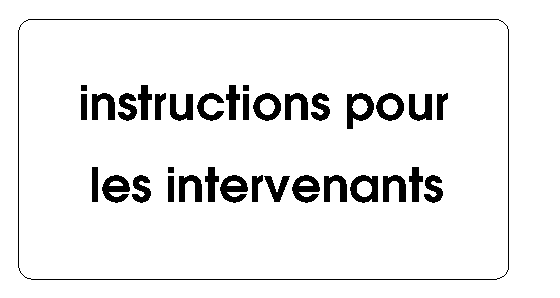
\includegraphics[width=10cm,angle=0]{guide_intervention_pg.eps}
\end{center}
\end{figure}
\end{center}
 \newpage

\tableofcontents


\section{Introduction}
  Merci de participer au projet {\sc Getfem++ / Getfem}. Ce projet a pour vocation la r\'ealisation d'un code interfac\'e avec MATLAB dans le domaine du calcul scientifique des EDP. Il s'ins\`ere dans le cadre de la formation en calcul scientifique du d\'epartement de G\'enie Math\'ematique et Mod\'elisation de l'INSA de Toulouse et du laboratoire MIP (math\'ematiques pour l'Industrie et la Physique).\\[0.4cm]
Ce guide a pour objectif de vous faciliter l'intervention sur le projet. Comme toutes les parties du projet, il est r\'evisable, et toute initiative visant \`a son am\'elioration est la bienvenue (r\'epertoire getfem++/doc/guide\_intervention/).

\newpage

\section{Organigramme simplifi\'e de GETFEM++}
GETFEM++ est un ensemble de biblioth\`eques C++ destin\'ees \`a donner un environnement le plus g\'en\'erique possible pour l'approximation par \'el\'ements finis (et m\'ethodes connexes) des probl\`emes mod\'elis\'es par des \'equations aux d\'eriv\'ees partielles. L'organigramme interne des diff\'erentes biblioth\`eques est donn\'e dans la figure qui suit.

\begin{center}
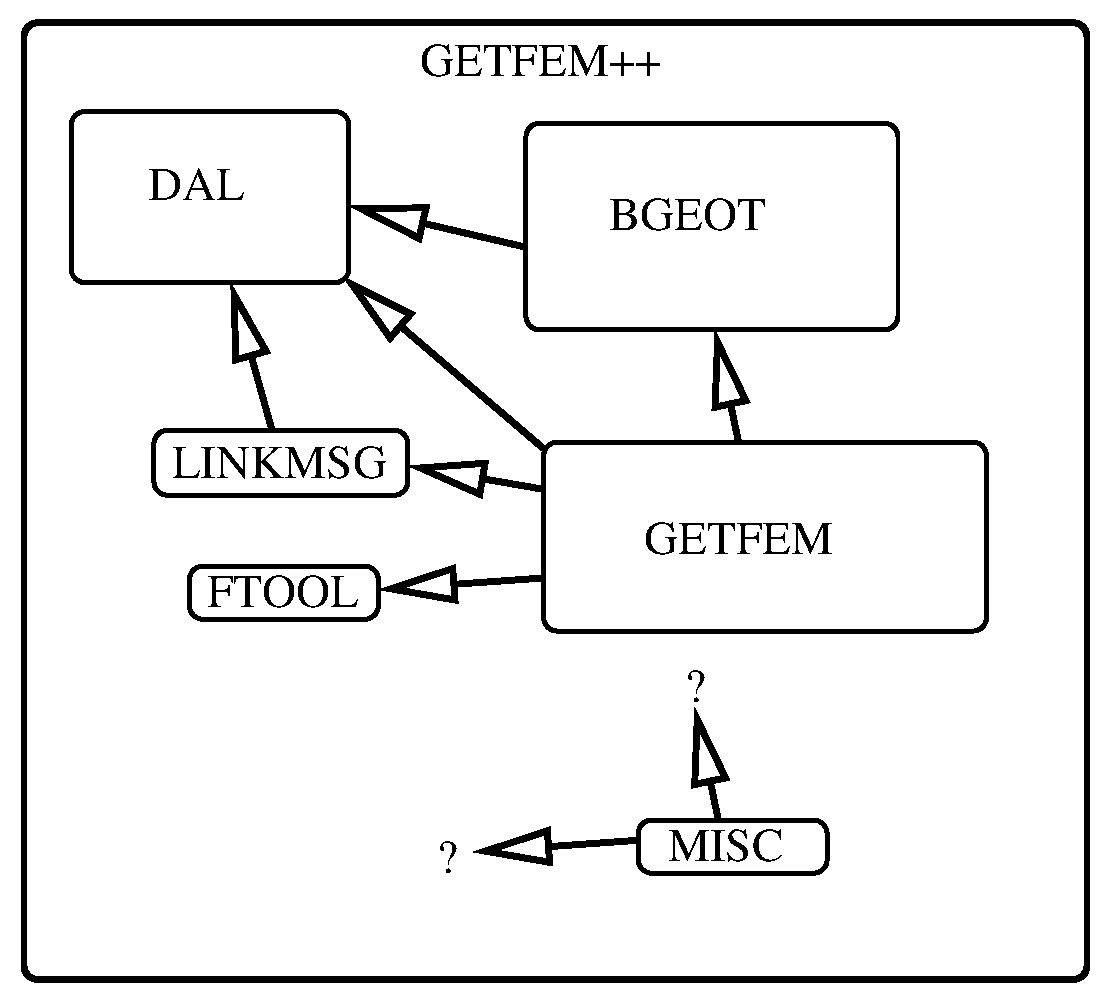
\includegraphics[width=17cm,angle=0]{getfem_orga.eps}
\end{center}
% $\;$\\[1cm]

Les diff\'erentes biblioth\`eques :
\begin{itemize}
  \item DAL : (Dynamic Array Library) c'est la biblioth\`eque de base du projet qui assure \`a la fois
    les probl\`emes de compatibilit\'e \'eventuels entre les diff\'erentes configurations et la d\'efinition de type {\bf container \'etendus} par rapports \`a la STL (Standard Template Library du C++). Ces types sont destin\'es \`a simplifier la programmation du reste du code, en particulier la gestion de maillage.\\[0.2cm]
  \item FTOOL : tr\`es petite biblioth\`eque de traitement de cha\^\i ne de caract\`eres.\\[0.2cm]
  \item LINKMSG : tr\`es petite biblioth\`eque de gestion de message entre objets.\\[0.2cm]
  \item BGEOT : (Basic Geometric Tool) diverses description g\'eom\'etriques (points, vecteurs, matrices, tenseurs, convexes, maillages \'el\'ementaires, polyn\^omes de plusieurs variables, d\'efinition d'\'el\'ements finis).\\[0.2cm]
  \item GETFEMLIB : (GEneric Tool for Finite Element Methods Library) Maillage permettant la gestion \'el\'ement finis, description des m\'ethodes d'\'el\'ements finis, m\'ethodes d'assemblage. \\[0.2cm]
  \item MISC : Partie du projet recevant les algorithmes r\'ecents et non organis\'es en biblioth\`eques. Les algorithmes de r\'esolutions sont pour le moment rang�s ici. Certaines parties de cet ensemble de fichiers sont destin\'es � dispara\^\i tre. \\[0.2cm]
\end{itemize}

\section{Futur organigramme simplifi\'e de GETFEM}
GETFEM repr\'esentera une sur-couche de GETFEM++ compos\'ee de sources C - C++ faisant interface \`a des commandes MATLAB et de sources MATLAB.

\begin{center}
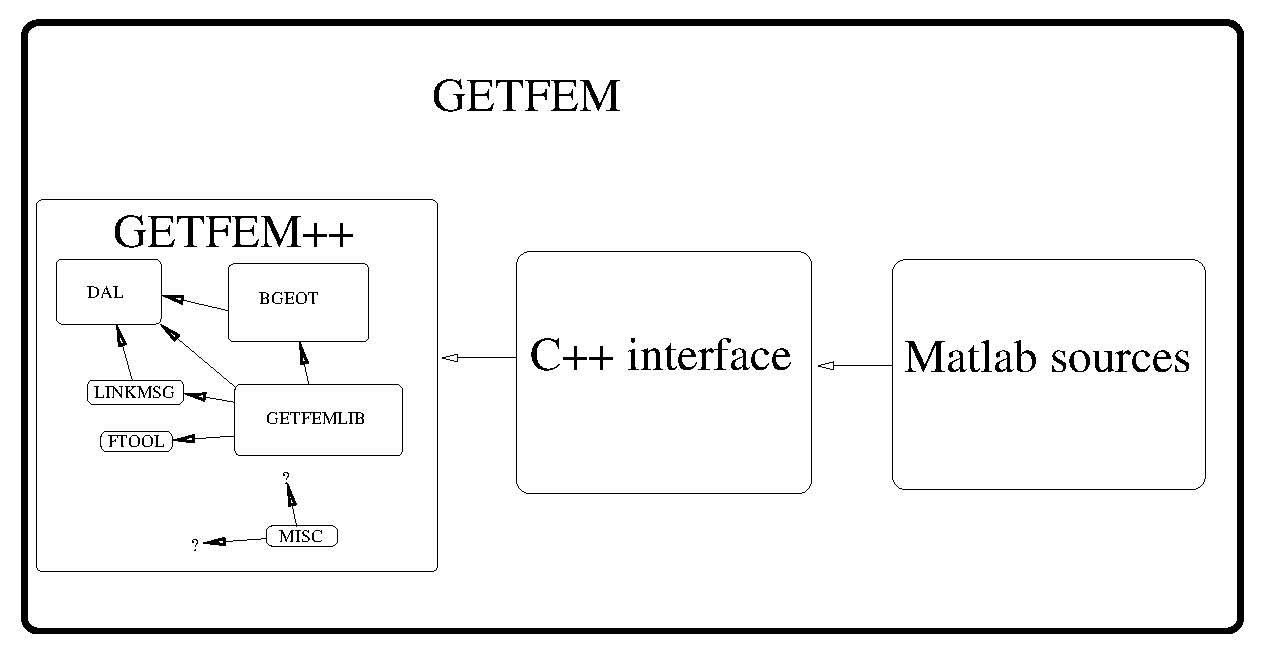
\includegraphics[width=17cm,angle=0]{getfemlab_orga.eps}
\end{center}

\section{Organisation du projet avec CVS}

\subsection{Introduction \`a CVS}
  CVS (Concurrent Versions System) permet la gestion des r\'evisions, ce qui est vital quand plusieurs programmeurs travaillent sur un m\^eme logiciel (et conseill\'e m\^eme pour un seul programmeur).\\[0.4cm]
L'id\'ee de base de CVS est de centraliser sur un unique r\'epertoire, dit d\'epot, soit repository en anglais, tous les codes et documents relatifs au projet (dans le cas pr\'esent, ce r\'epertoire est sur gmmlinux2). Chaque intervenant travaille alors sur une copie des sources de la partie du projet sur laquelle il intervient.\\[0.4cm]
Des commandes permettent de tester la validit\'e de ces sources, de les mettre \`a jour par rapport aux changement effectu\'ees par d'autre sur le repository, de valider ses propres changements effectu\'es sur sa propre copie, ou d'ajouter et de supprimer des fichiers au projet.\\[0.4cm]
CVS g\`ere automatiquement l'attribution de num\'eros de r\'evision \`a chaque fichier du projet. Toutes les modifications sont gard\'ees en m\'emoire, de telle mani\`ere \`a ce que l'on puisse demander l'\'etat du projet \`a n'importe quelle date ant\'erieure. \\[0.4cm]
D'autres fonctionnalit\'es plus \'evolu\'ees existent, toutefois, dans la suite de ce guide, seule les commandes de base seront introduites.\\[0.4cm]
ATTENTION : Soyez bien s\^ur de vous lorsque vous apportez des modifications au repository, l'ensemble des autres intervenants les chargeront lors de leurs prochaines interventions. Il est imp\'eratif d'\'eviter au maximum d'introduire de nouvelles erreurs dans le projet. 

  
\subsection{Structure des fichiers du projet sous CVS}

\begin{center}
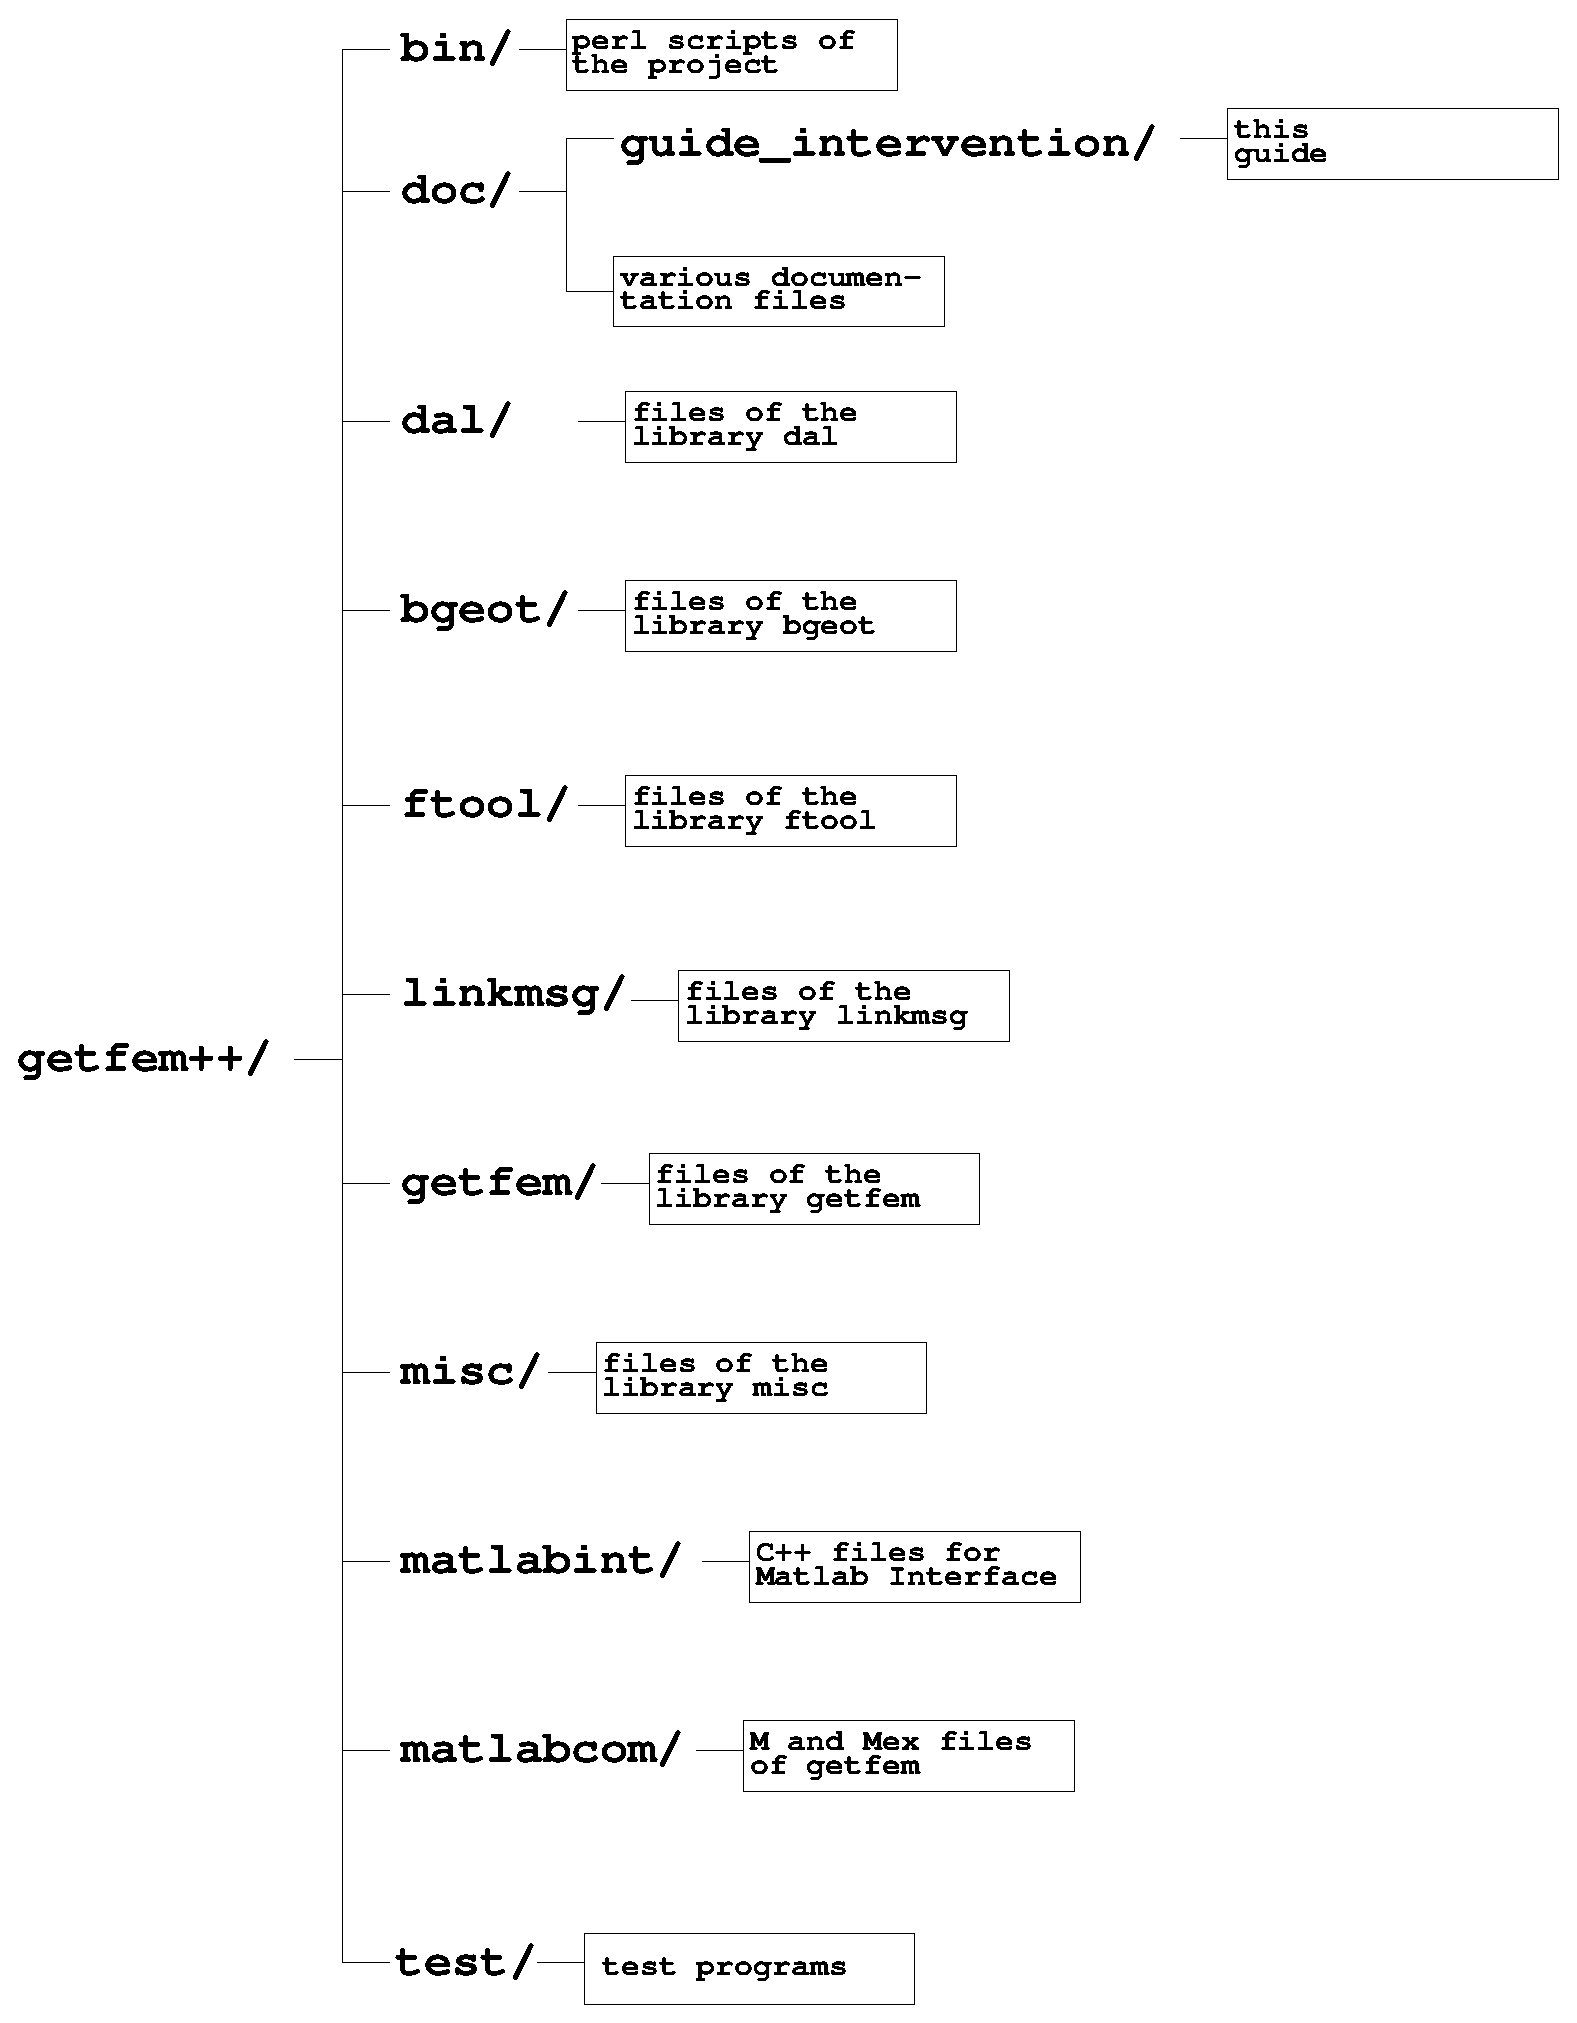
\includegraphics[width=17cm,angle=0]{files_structure.eps}
\end{center}

\section{R\'ecup\'erer et mettre \`a jour des fichiers avec CVS}
\subsection{Initialisation}
On doit tout d'abord initialiser la variable CVSROOT par la commande
\begin{alltt} setenv CVSROOT :pserver:nom_login@gmmlinux2.gmm.priv:/var/cvs
\end{alltt}
pour csh, o\`u
\begin{alltt} export CVSROOT=:pserver:nom_login@gmmlinux2.gmm.priv:/var/cvs
\end{alltt}
pour bash, o\`u nom\_login est votre nom de login unix sur le site du gmm. cette commande peut \^etre ins\'er\'ee dans votre .cshrc, .bashrc ou autre. 

\subsection{R\'ecup\'erer une partie des sources}
D'une mani\`ere g\'en\'erale, r\'ecup\'erer des sources s'op\`ere par la commande
\begin{alltt}
  cvs checkout nom_dir
\end{alltt}
o\`u nom\_dir est le nom du r\'epertoire a rapatrier (voir structure des fichiers du projet sous CVS).
Par exemple la commande
\begin{alltt}
  cvs checkout getfem++/dal/test
\end{alltt}
va cr\'eer dans le r\'epertoire courant la structure de r\'epertoire \begin{alltt} getfem++/dal/test/ \end{alltt} et y mettre les fichier correspondants, c'est \`a dire les programmes de test de la biblioth\`eque dal.

\subsection{Plus pratique, les shells d'installation et de mise \`a jour}
Les shells d'installation et de mise \`a jour regroupent toutes les instructions permettant de r\'ecup\'erer la partie des sources que vous souhaitez modifier, et d'installer un environnement de compilation et de test. Pour r\'ecup\'erer l'ensemble des shells d'installation, ex\'ecuter la commande
\begin{alltt}
  cvs checkout getfem++/bin
\end{alltt}
Cette commande rapatrie en fait tout les shells ex\'ecutables du projet getfem++. Entrer alors dans le r\'epertoire getfem++ ainsi cr\'ee par
\begin{alltt} cd getfem++ \end{alltt}
et taper
\begin{alltt} 
  bin/startdal, bin/startbgeot, bin/startgetfem,
  bin/startftool, bin/startlinkmsg, bin/startmisc,
  bin/startmatlab_interface, ou bin/startgetfemlab
\end{alltt}
ces shells chargent l'int\'egralit\'e des biblioth\`eques consid\'er\'ees et pr\'eparent un makefile pour compiler celles-ci, ainsi que les programmes de test qui lui sont li\'es. Vous pouvez encha\^\i ner plusieurs shells si vous voulez intervenir sur plusieurs biblioth\`eques dans la m\^eme session, ou si vous n'allez tester les modifications apport\'ees dans des biblioth\`eques autre que celle que vous modifiez.\\[0.4cm]

Une fois les modifications apport\'ees, il faut passer \`a une phase de test, i.e. compilation et lancement des programmes de tests. Si la partie que vous avez modifi\'ee n'a pas de programme de test correspondant, cr\'eez-en un, en essayant de tester toutes les fonctionnalit\'es.\\[0.4cm]

Une fois la phase de test compl\'et\'ee, quand vous \^etes s\^ur que vous n'introduisez pas de nouveaux bugs dans le projet, validez les changements en ex\'ecutant
\begin{alltt}
  cvs commit -m "commentaire"
\end{alltt}
Attention, soyez bien s\^ur de la validit\'e de vos changements avant de taper ces commandes. Les modifications seront imm\'ediatement transf\'er\'ees dans le repository. Les changements dans les sources compilables seront pris en compte dans une recompilation de la biblioth\`eque qui a lieu toutes les nuits.\\ \\

D'une mani\`ere g\'en\'erale, ne gardez pas trop longtemps ouverte une session. Une fois la commande ``cvs commit'' effectu\'ee, vous pouvez d\'etruire le r\'epertoire. \\ \\

\underline{exemple de session de modification, test, et validation}
\begin{largebox}
\begin{alltt}
  cvs checkout getfem++/bin
  cd getfem++
  bin/startbgeot
  xemacs bgeot/bgeot_poly.h (+ modifications)
  make
  make test
  cvs commit -m "la modification que j'ai apport\'ee concerne ..."
  cd ..
  /bin/rm -r getfem++
\end{alltt}
\end{largebox}


\subsubsection{Ajouter un fichier au projet}

Pour ajouter un nouveau fichier au projet, il faut tout d'abord charger le r\'epertoire ou ce fichier doit \^etre ajout\'e par une commande du type \begin{alltt} cvs checkout \end{alltt}.
Il faut alors se positionner sur ce r\'epertoire, cr\'eer ce nouveau fichier, puis ex\'ecuter la commande
\begin{alltt}
  cvs add nom_fichier
\end{alltt}
Cette commande doit obligatoirement \^etre ex\'ecut\'ee dans le r\'epertoire ou est cr\'ee le fichier. On ne peut faire de commande du style ``cvs add getfem++/dal/nouveau-fichier.h''.
Une fois cela fait, on peut encore modifier le fichier, et il faut terminer la session par un
\begin{alltt}
  cvs commit -m "commentaire"
\end{alltt}
pour valider l'ajout de fichier.

\subsubsection{Supprimer un fichier au projet}
Comme pour l'ajout, on doit tout d'abord charger le r\'epertoire ou ce fichier existe, puis se positionner dessus. On doit alors supprimer ce fichier par une commande
\begin{alltt}
  rm nom_fichier
\end{alltt}
puis ex\'ecuter la commande
\begin{alltt}
  cvs remove nom_fichier
\end{alltt}
L\`a aussi, il faut valider l'op\'eration par un
\begin{alltt}
  cvs commit -m "commentaire"
\end{alltt}


\section{charte de programmation}

 \subsection{Sources C++}
   on veillera \`a respecter les points suivants :
   \begin{itemize}
     \item Ne pas oublier de commenter les sources, et de les documenter (voir section suivante)
     \item Dans les biblioth\`eques, \`a tout fichier .C doit correspondre un fichier .h m\^eme succinct.
     \item respecter la mise en forme des fichiers sources telle qu'elle existe actuellement.
   \end{itemize}
   \`a compl\'eter

 \subsection{Sources Matlab}
   on veillera \`a respecter les points suivants :
   \begin{itemize}
     \item Ne pas oublier de commenter les sources, et de les documenter (voir section suivante)
   \end{itemize}
   \`a compl\'eter
\section{charte de documentation}
  Les documentations sont \`a r\'ealiser en anglais.
  \subsection{Documentation des sources C et C++}
  Le choix s'est port� sur un outils de documentation automatique des sources. Il s'agit du logiciel DOC++ (http::\/\/docpp.sourceforge.net). Son utilisation est simple et consiste � documenter dans les sources C ou C++ (voir aussi la doc dans getfem++/doc/doc++.ps). Pour cela deux types de commentaires peuvent �tre introduits. Sur une seule ligne par :\\
{\tt
 /// comment
}
\\ ou sur plusieurs lignes par :
\begin{alltt}
/** comment 1 
 *  comment 2 
 *  comment 3 
 */ 
\end{alltt}
Ces commentaires doivent pr�ceder directement les �l�ments � commenter (fonctions, classes, m�thodes d'une classe). Se reporter aux modules correctement commenter pour avoir une id�e des formats.
on veillera \`a respecter les points suivants :
   \begin{itemize}
     \item Essayer de commenter toutes les classes, fonctions, m�thodes, et en priorit� les �l�ments exportables.
     \item Donner tout les �l�ments n�cessaire � la compr�hension du module. En r�gle g�n�rale, on fournira des informations extensive que l'on rattachera � la classe principale du module (m�thode de calcul, calcul int�rm�diaires, d�tails d'impl�mentation ...)
     \item Donner si possible quelques exemples d'utilisation des classes.
   \end{itemize}
  \subsection{Documentation des sources Matlab}
  \`a compl\'eter
  \subsection{Documentation des exemples d'application}
  \`a compl\'eter

\end{document}
